\documentclass[tikz,border=4pt]{standalone}
\usepackage{tikz}
\usetikzlibrary{arrows.meta,calc}
\begin{document}
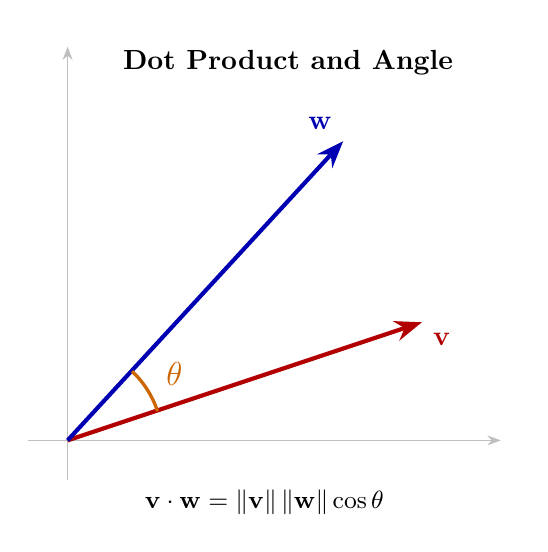
\begin{tikzpicture}[
    >=Stealth,
    axis/.style={->,gray!50},
    vec/.style={->,line width=1.5pt},
]
\node[font=\bfseries] at (2.8,4.8) {Dot Product and Angle};

\draw[axis] (-0.5,0) -- (5.5,0) node[right,font=\small] {};
\draw[axis] (0,-0.5) -- (0,5) node[above,font=\small] {};

% Vector v (lower, more horizontal)
\draw[vec,red!70!black] (0,0) -- (4.5,1.5)
    node[below right,font=\bfseries] {$\mathbf{v}$};

% Vector w (upper, steeper)
\draw[vec,blue!70!black] (0,0) -- (3.5,3.8)
    node[above left,font=\bfseries] {$\mathbf{w}$};

% Angle arc
\draw[orange!80!black,line width=1.2pt]
    (0,0) ++(18:1.2) arc (18:47:1.2);
\node[orange!80!black,font=\large] at (32:1.6) {$\theta$};

% Formula
\node[font=\small,anchor=north] at (2.5,-0.5)
    {$\mathbf{v}\cdot\mathbf{w} = \|\mathbf{v}\|\,\|\mathbf{w}\|\cos\theta$};
\end{tikzpicture}
\end{document}
